%the shimmer device
\section{Instrumentation} \label{methods:instrumentation}

For this project data will be acquired using accelerometers, gyroscopes and force sensors. The accelerometer and/or gyroscopes is provided through the use of the Shimmer3 device from ShimmerSensing. Force sensors are from Interlink Electronics of the 400 Series. %Data will be collected using MATLAB. 

The Shimmer3 device is a nine degree of freedom (DoF) Inertial Measurement Unit (IMU) possessing five different types of sensors; accelerometer, gyroscope, magnetometer and altimeter. The Shimmer3 is capable of being configured to enable or disable specific sensors depending on which is needed. For this project only the accelerometer and gyroscope modules of the device will be used. The Shimmer3 device has two accelerometers, a wide range and a low noise. The wide range accelerometer is of the component LSM303DLHC. It has a three dimensional digital linear acceleration sensor with a range of $\pm$2g / $\pm$4g / $\pm$8g / $\pm$16g, and sensitivity of 1000 Least Significant Bit (LSB) per g at $\pm$2g. \cite{LSM303DLHC, ShimmerSensing2016} % The LSM303DLHC also features a magnometer.  %It has 16bit data output and communicates through an I$^{2}$C serial interface.
The low noice accelerometer is a KXRB5-2042 with a range of $\pm$2g. The sensitivity is 600$\pm$18 mV/g. \cite{ShimmerSensing2016}
The gyroscope in the Shimmer3 device is a MPU-9150, with a range of $\pm$250 / $\pm$500 / $\pm$1000 / $\pm$2000 degrees per second (dps). The gyroscope has sensitivity of 131 LSB/dps at $\pm$250dps. \cite{ShimmerSensing2016}
Communication between the Shimmer3 devices and the computer is through Bluetooth. The computer will be running MATLAB and the \textit{Shimmer MATLAB Instrument Driver Library} to collect the streamed data from the Shimmer3 device. 
The Shimmer3 device has dimensions of 51mm x 34mm x 41mm and is easy to place nearly anywhere on the body with elastic straps with snap clips. Two Shimmer3 devices will be used for this project. 

%SHIMMER3 DEVICE BODY POSITION PLACEMENT: One device will be mounted on the head of the subject, one at the chest and one at the waist. 

The force sensors used in this project are Force Sensing Resistors (FSR) from Interlink Electronics, models 402 and 406. The FSR 402 is a 13mm diameter circle single-zone resistor capable of force detection in a range from 20g to 2kg. The FSR 406 is similar but covers a larger area of 38mm in a square. \cite{IE400} A total of six sensors will be used with three sensors under each foot. 
An Arduino Uno will be used for handling recording and saving the data from the FSRs. The Arduino Uno is mounted on a breadboard, and connected to six jack stick plugs, an SD-card reader and battery holder for power supply (see \figref{fig:breadboardSetup}). The FSRs are connected to the Arduino Uno through 3.5mm jack sticks. 
%[foot regions: https://www.sciencephoto.com/media/581111/view/anatomy-regions-of-the-right-foot]
%(https://www.digikey.ca/product-detail/en/interlink-electronics/30-73258/1027-1002-ND/2476470) big square sensor
%(https://www.digikey.ca/product-detail/en/interlink-electronics/30-81794/1027-1001-ND/2476468) small round sensor

\begin{figure}[H]
	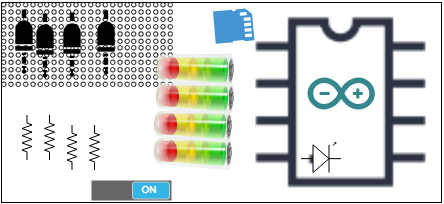
\includegraphics[width=.6\textwidth]{figures/breadboardSetup}
	\caption{The setup of the breadboard used for data collection from the FSRs on the feet.}
	\label{fig:breadboardSetup}  %<--remember LABEL!
\end{figure}





